
%(BEGIN_QUESTION)
% Copyright 2010, Tony R. Kuphaldt, released under the Creative Commons Attribution License (v 1.0)
% This means you may do almost anything with this work of mine, so long as you give me proper credit

Calculate the amount of energy stored in each of the reactive elements (inductor, capacitor), assuming enough time has passed for voltage and current to reach their ``final'' values in these devices:

$$\includegraphics[width=15.5cm]{i02512x01.eps}$$

\vfil

\underbar{file i02512}
\eject
%(END_QUESTION)





%(BEGIN_ANSWER)

This is a graded question -- no answers or hints given!

%(END_ANSWER)





%(BEGIN_NOTES)

Energy storage in an inductor is a function of the current through that inductor.  Therefore, we must first solve for inductor current.  Assuming the inductor contains zero resistance, and the only limit to maximum current in this circuit will be the resistor, we may calculate the current using Ohm's Law.  A 15 VDC source and a 3.3 k$\Omega$ resistor yields a current of 4.545 mA:

$$E_L = {1 \over 2} L I^2$$

$$E_L = {1 \over 2} (0.075) (0.004545)^2$$

$$E_L = 774.79 \hbox{ nJ}$$

\vskip 30pt

Energy storage in a capacitor is a function of the voltage across that capacitor.  Therefore, we must first solve for capacitor voltage.  We may do this by applying the voltage divider formula to the two resistors in this circuit, calculating the voltage across the 1.2 k$\Omega$ resistor.  With a 25 VDC supply, we get 6.667 volts:

$$E_C = {1 \over 2} C V^2$$

$$E_C = {1 \over 2} (47 \times 10^{-6}) (6.667)^2$$

$$E_C = 1.0444 \hbox{ mJ}$$

%INDEX% Electronics review: energy stored in a capacitor
%INDEX% Electronics review: energy stored in an inductor

%(END_NOTES)


